% 由 render.py 自动生成，请勿手改——改 paper.tex 或 facts.json 后重跑。
% source: C:\Users\ROG\Desktop\DeepSeek\math-modeling-cumcm\examples\demo\paper\paper.tex

% !TEX program = xelatex
% ============================================================
% 国赛论文模板（CUMCM）
% 编译：xelatex paper.rendered.tex（跑两遍以更新交叉引用）
% 先用 python scripts/render.py 渲染占位符，再编译。
% ============================================================
\documentclass[UTF8,12pt,fontset=windows]{ctexart}

\usepackage{amsmath,amssymb}
\usepackage{graphicx}
\usepackage{booktabs}
\usepackage{array}
\usepackage{geometry}
\usepackage{xcolor}
\usepackage{caption}
\usepackage{float}
\usepackage[hidelinks]{hyperref}

\geometry{a4paper, margin=2.5cm}
\linespread{1.5}
\captionsetup{font=small, labelsep=quad}

% ---- 自定义命令 ----
% 结果占位符：渲染脚本会替换为 facts.json 中的数值；未渲染时显示红色 ??key??
\newcommand{\res}[1]{\textcolor{red}{\textbf{??#1??}}}
% AI 使用标注角标
\newcommand{\aiflag}[1]{\textsuperscript{\textcolor{gray}{[AI#1]}}}
% 待人工补充标记
\newcommand{\todomark}[1]{\textcolor{orange}{\textbf{[TODO: #1]}}}

\title{\zihao{3}\heiti 基于\underline{\quad\quad}的\underline{\quad\quad}模型}
\author{}
\date{}

\begin{document}

% ==================== 摘要页 ====================
\begin{center}
{\zihao{3}\heiti 基于\underline{\quad\quad}的\underline{\quad\quad}模型}
\end{center}

\vspace{0.5em}
\begin{center}
{\zihao{4}\heiti 摘\quad 要}
\end{center}

% TODO(人工): 摘要四段式——背景一句 + 每问"方法→结果(带数字)" + 检验结论 + 评价一句。
% 每问必须有结论性数字，数字一律用 \res{key}。
针对问题一，……，得到 0.0421。\aiflag{1}

针对问题二，……，得到最优总成本 1,234.56 万元，较基准方案下降 17.7\%。

针对问题三，……

模型检验表明，……结论对参数扰动不敏感。

本文模型的优点在于……，可推广至……

\vspace{0.8em}
\noindent\textbf{关键词：}\quad ……；……；……；……

\newpage

% ==================== 目录（可选） ====================
% \tableofcontents
% \newpage

% ==================== 一、问题重述 ====================
\section{问题重述}

\subsection{问题背景}
% TODO(人工): 用自己的话改写，不得整段抄题。
……

\subsection{需要解决的问题}
\begin{enumerate}
  \item \textbf{问题一}：……
  \item \textbf{问题二}：……
\end{enumerate}

% ==================== 二、问题分析 ====================
\section{问题分析}

% TODO(人工): 每问的目标/已知/缺口/难点，并画技术路线图。
……

\begin{figure}[H]
  \centering
  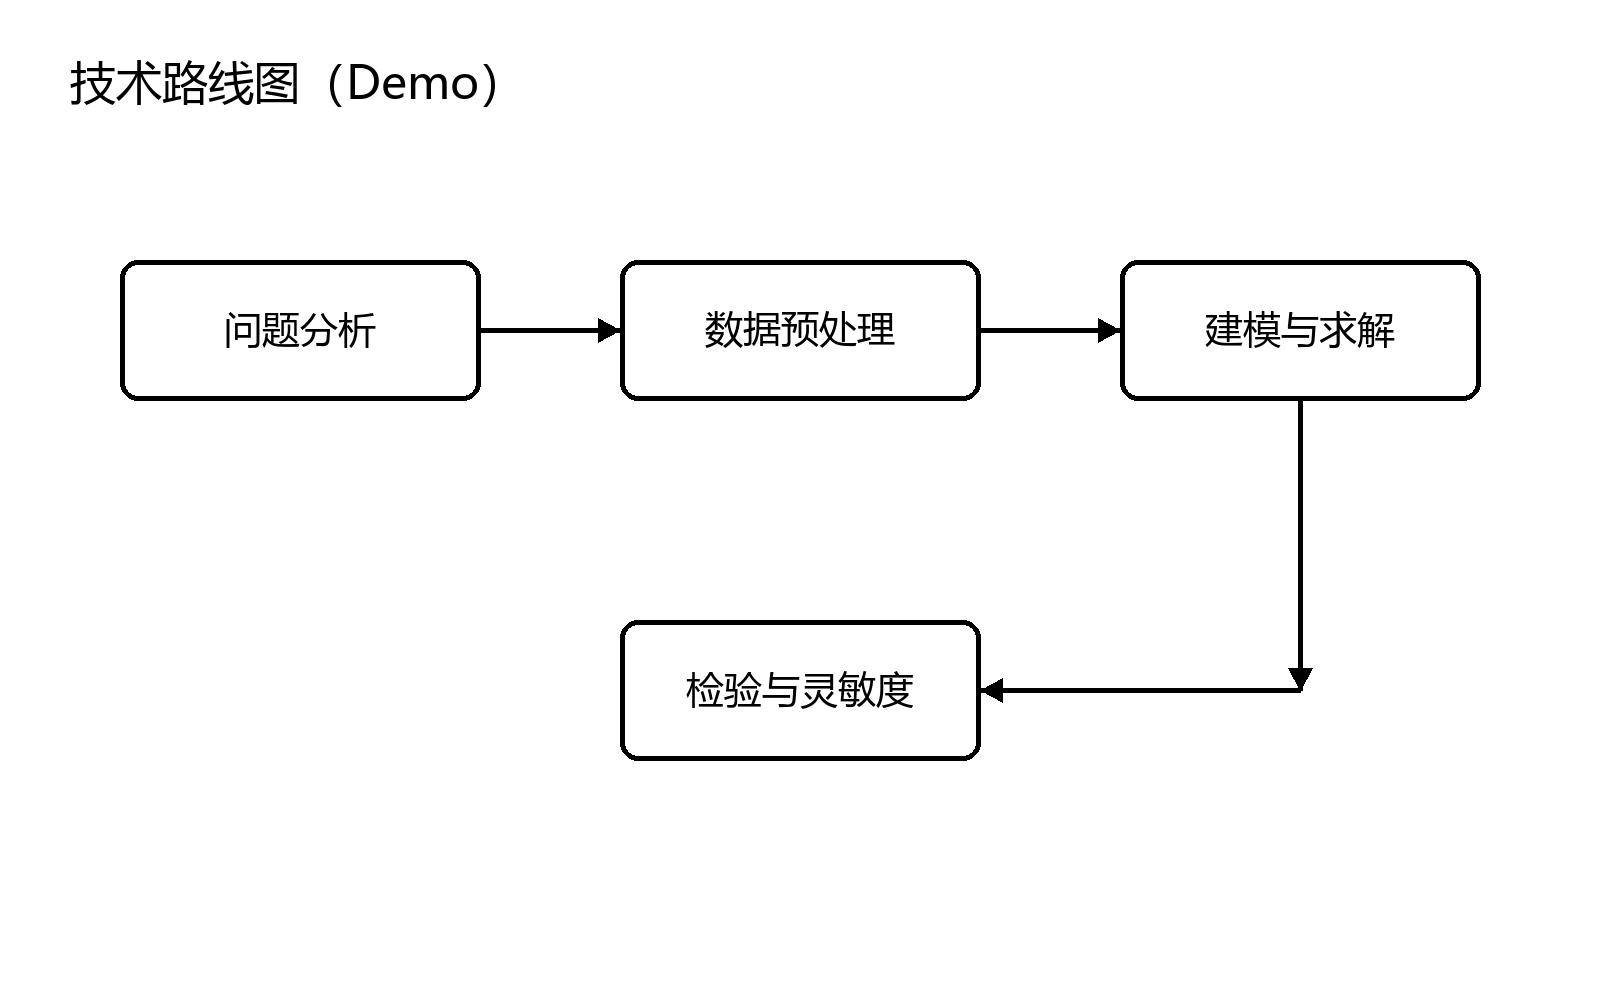
\includegraphics[width=0.8\textwidth]{figs/roadmap.pdf}
  \caption{技术路线图}\label{fig:roadmap}
\end{figure}

% ==================== 三、模型假设 ====================
\section{模型假设}

\begin{enumerate}
  \item \textbf{假设一}：……。\textbf{理由：}……。\textbf{放宽影响：}……。
\end{enumerate}

% ==================== 四、符号说明 ====================
\section{符号说明}

\begin{table}[H]
  \centering
  \caption{符号说明}
  \label{tab:symbols}
  \begin{tabular}{ccc}
    \toprule
    符号 & 含义 & 单位 \\
    \midrule
    $x_i$ & …… & —— \\
    \bottomrule
  \end{tabular}
\end{table}

% ==================== 五、模型建立与求解 ====================
\section{模型建立与求解}

\subsection{问题一模型的建立}

……

\begin{equation}
  \min\ Z = \sum_{i=1}^{n} c_i x_i
  \label{eq:q1-obj}
\end{equation}

\subsection{问题一模型的求解}

……

\begin{table}[H]
  \centering
  \caption{问题一求解结果}
  \label{tab:q1-result}
  \begin{tabular}{ccc}
    \toprule
    方案 & 目标值 & 备注 \\
    \midrule
    本文方法 & 0.0421 & …… \\
    \bottomrule
  \end{tabular}
\end{table}

如表 \ref{tab:q1-result} 所示，……。

\subsection{问题二模型的建立与求解}

……

% ==================== 六、模型检验 ====================
\section{模型检验}

\subsection{灵敏度分析}
% TODO(人工): 至少一个参数扰动，给出数值与结论。
当参数 $\alpha$ 上浮 10\% 时，目标值变化率为 0.031，说明……。% nofact: 10\% 是实验设定输入值，非计算结果

\subsection{稳健性检验}
……

% ==================== 七、模型评价与推广 ====================
\section{模型评价与推广}

\subsection{模型优点}
\begin{enumerate}
  \item ……（要具体，如"计算复杂度 $O(n\log n)$，可实时"）
\end{enumerate}

\subsection{模型缺点}
\begin{enumerate}
  \item ……（要诚实，如"依赖数据平稳性假设"）
\end{enumerate}

\subsection{模型推广}
……

% ==================== 参考文献 ====================
\begin{thebibliography}{99}
\bibitem{ref1} 作者. 题名[M]. 出版地: 出版社, 年.
% AI 工具条目（按官方格式；版本写实际调用模型）
\bibitem{ai1} DeepSeek, deepseek-chat, 深度求索（DeepSeek）, 2025-09-05.
\end{thebibliography}

% ==================== 附录 ====================
\newpage
\appendix
\section{附录：程序代码}

% TODO(人工): 贴入完整可运行代码，按问题分节，注明依赖与随机种子。
\begin{verbatim}
# code/solve_q1.py
\end{verbatim}

\end{document}
